\section{Концепция требований}\label{COMMON.Concept}

Требования настоящего стандарта направлены на достижение трех целей, 
определяемых ниже. Каждая цель задает направление усиления
требований безопасности. При движении по направлению выполняются переходы с
уровня на уровень.

Среда эксплуатации СКЗИ является потенциальным источником угроз и атак. 
%
% Разработчик СКЗИ не должен делать предположений о том, что находится за 
% границей. Но он может делать предположения о том, что находится в пределах 
% границы.
%
Первая цель~--- защита криптографической границы, отделяющей СКЗИ от среды
(см.~рис.~\ref{Fig.COMMON.Concept}).
%
Направления защиты:
\begin{itemize}
\item
физическая защита от проникновения;
\item
логическая защита (аутентификация);
\item
защита от побочных каналов (т.~е. передачи данных за пределы границы).
\end{itemize}

\begin{figure}[bht]
\begin{center}
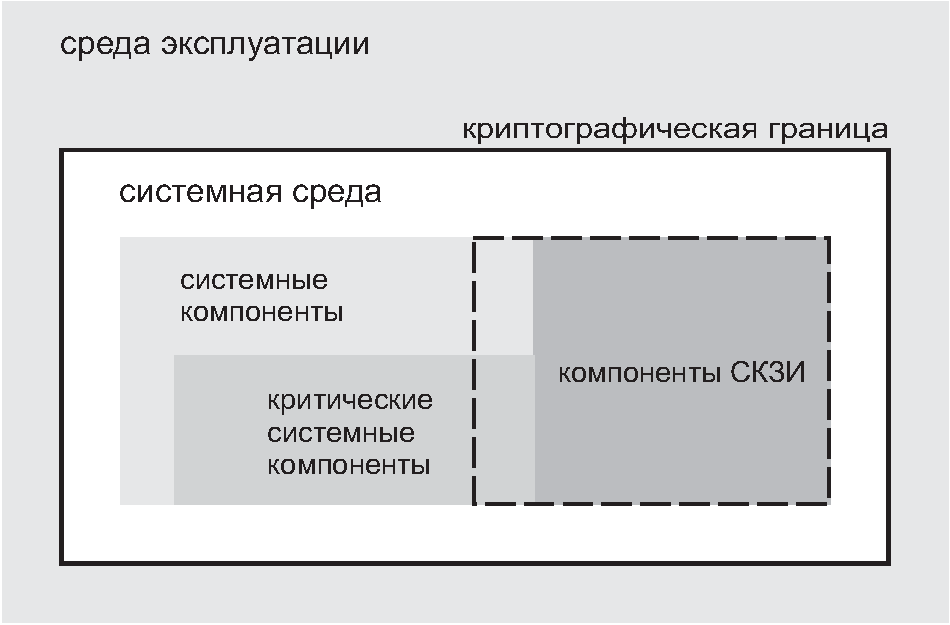
\includegraphics[width=11cm]{../figs/env}
\end{center}
\caption{Среды и компоненты}\label{Fig.COMMON.Concept}
\end{figure}

Область в пределах криптографической границы~--- системная среда~---
включает системные компоненты. Это процессор, устройства хранения, 
устройства сопряжения, операционная система, другие СКЗИ. 
%
Среди системных компонентов выделяются критические~--- те, от которых зависит  
работоспособность и безопасность СКЗИ. 

Системный компонент может входить в состав СКЗИ или быть внешним по отношению
к средству. Например, процессор входит в состав аппаратного СКЗИ и не входит в 
состав программного. 
%
Компонент классифицируется как системный, если он создается без связи с 
СКЗИ, а при разработке СКЗИ только интегрируется и возможно конфигурируется.
%
Системные компоненты как правило являются массовыми, предназначенными для 
широкого круга потребителей, и универсальными, не ориентированными на 
реализацию исключительно криптографических сервисов.

Системный компонент, в том числе критический, является не до конца доверенным. 
% 
Факторы неполного доверия:
%
непрозрачность закрытых (проприетарных) компонентов,
%
сложность и сопутствующие ей ошибки при разработке,
%
модифицируемость с непредсказуемым поведением после модификации,
%
одновременный доступ к компонентам нескольких операторов с риском раскрытия или 
подмены объектов друг друга,
%
сбои в аппаратных компонентах,
%
другое.

Вторая цель требований безопасности~--- повышение доверия к КСК. 
Направления защиты:
\begin{itemize}
\item
контроль состава КСК;
\item
контроль работоспособности КСК;
\item
настройка параметров безопасности КСК;
\item
контроль статуса безопасности КСК (учет известных уязвимостей);
\item
оценка безопасности пограничных КСК, реализующих интерфейсы взаимодействия со 
средой эксплуатации.
\end{itemize}

Криптографическая граница определяется разработчиком.
В большинстве случаев определяется однозначно и естественно:  
физический контур аппаратного средства или периметр корпуса персонального 
компьютера с установленным на нем программным средством.
%
Если имеется свобода при определении границы, то разработчик может
воспользоваться ею, либо делая акцент на защиту границы, либо отодвигая границу
от средства и расширяя таким образом системную среду. В последнем случае
потребуется взять под контроль дополнительные КСК.

Собственные компоненты СКЗИ размещаются в системной среде вместе с системными.
Примеры программных собственных компонентов: 
встроенное программное обеспечение (<<прошивки>>),
криптографические библиотеки, конфигурационные файлы, криптографические 
контейнеры.
%
Примеры аппаратных: печатные платы, источники энтропии.

Третья цель требований безопасности~--- надежность и качество собственных 
компонентов СКЗИ.
%
Направления:
\begin{itemize}
\item 
надежные криптографические алгоритмы;
\item 
надежные механизмы безопасности;
\item 
надежное криптографическое проектирование;
\item 
полномасштабный анализ исходных текстов;
\item 
полномасштабное тестирование;
\item 
безопасный жизненный цикл;
\item 
подробные руководства.
\end{itemize}
